\documentclass{TDP005mall}

\newcommand{\version}{Version 1.0}
\author{Love Jansson, \url{lovja643@student.liu.se}\\
  Charlie Simonsson, \url{chasi127@student.liu.se}}
  
\title{Comet Raids - Designspecifikation}
\date{2019-12-19}
\rhead{Love Jansson \\ Charlie Simonsson}
\usepackage[final]{pdfpages}
\usepackage{hyperref}

\begin{document}
\projectpage
\section{Revisionshistorik}
\begin{table}[!h]
\begin{tabularx}{\linewidth}{|l|X|l|}
\hline
Ver. & Revisionsbeskrivning & Datum \\\hline
0.1 & Kopierat från mall & 191129 \\\hline
0.2 & Första utkast & 191129 \\\hline
1.0 & Klar & 191219 \\\hline
\end{tabularx}
\end{table}

\tableofcontents

\pagebreak

\section{Inledning}
Detta dokument innehåller en specifikation av klassstrukturen för
spelet Comet Raids. Inledningsvis beskrivs den metod som tillämpats för att skapa
designen av spelet och därefter förklaras designen. Slutligen framförs en 
diskussion av systemets för- och nackdelar samt vilka externa filformat som används.\\

\subsection{Designmetod}
Den övergripande designen av spelet är objektorienterat.
Framtagningen av klasserna har skett enligt metoden objektorienterad analys(OOA)
följt av en objektorienterad design(OOD). Inledningsvis diskuterades vilka
objekt spelet skulle bestå av och baserat på resultatet framtogs klasser. Sedan
identifierades relationer mellan klasserna och hur den övergripande
klasstrukturen skulle se ut. Under programmeringsfasen användes en 
iterativ designfilosofi vilket ledde till förändringar från originalklasstrukturen.
Dessa förändringar kommer diskuteras mer i slutet av dokumentet.

\subsection{Övergripande design}
Spelet består av tre huvudsakliga klasser Object, State och Constants. Dessa klasser
inkluderas i en Main fil vars ansvar är att kalla funktionen run som i sin tur är
definierad i samma fil. Denna funktion initierar spelets grafik motor och skapar det
initiala State som visas, detta State är Start menyn vilket är en instans av MenuState.  

Klassen State ligger högst upp i en hierarki av tillstånd som spelet kan köras i.
Det finns två huvudtillstånd, GameState och MenuState. MenuState i sin tur har två
olika underklasser som heter PausMenuState och WinMenuState. GameState ansvarar för att
hanteringen av alla Object instanser och kör deras update funktioner samt kontrollerar
om dessa Object har kolliderat. GameState kontrollerar även om spelaren har vunnit
eller förlorat spelet och skickar programmet vidare till relevanta States beroende på
spelar input.
Spelets objekt ärver av en central klass som heter Object. Under Object i dess hierarki
ligger StaticObject och DynamicObject. StaticObject instanser är banan som spelaren
navigerar, de BombSites som spelaren ska släppa bomber på samt Explosioner som kommer när
en Bomb exploderar.
DynamicObject instanser inkluderar alla Object som kan ändra positioner under spelets
gång: Ship skeppet som spelaren styr, IceBlock, Bomb och Projectile.\\
\\
Nedan följer ett klassdiagram som visar en detaljerad översikt av programmets klasstruktur.
\pagebreak

\begin{figure}[h!]
  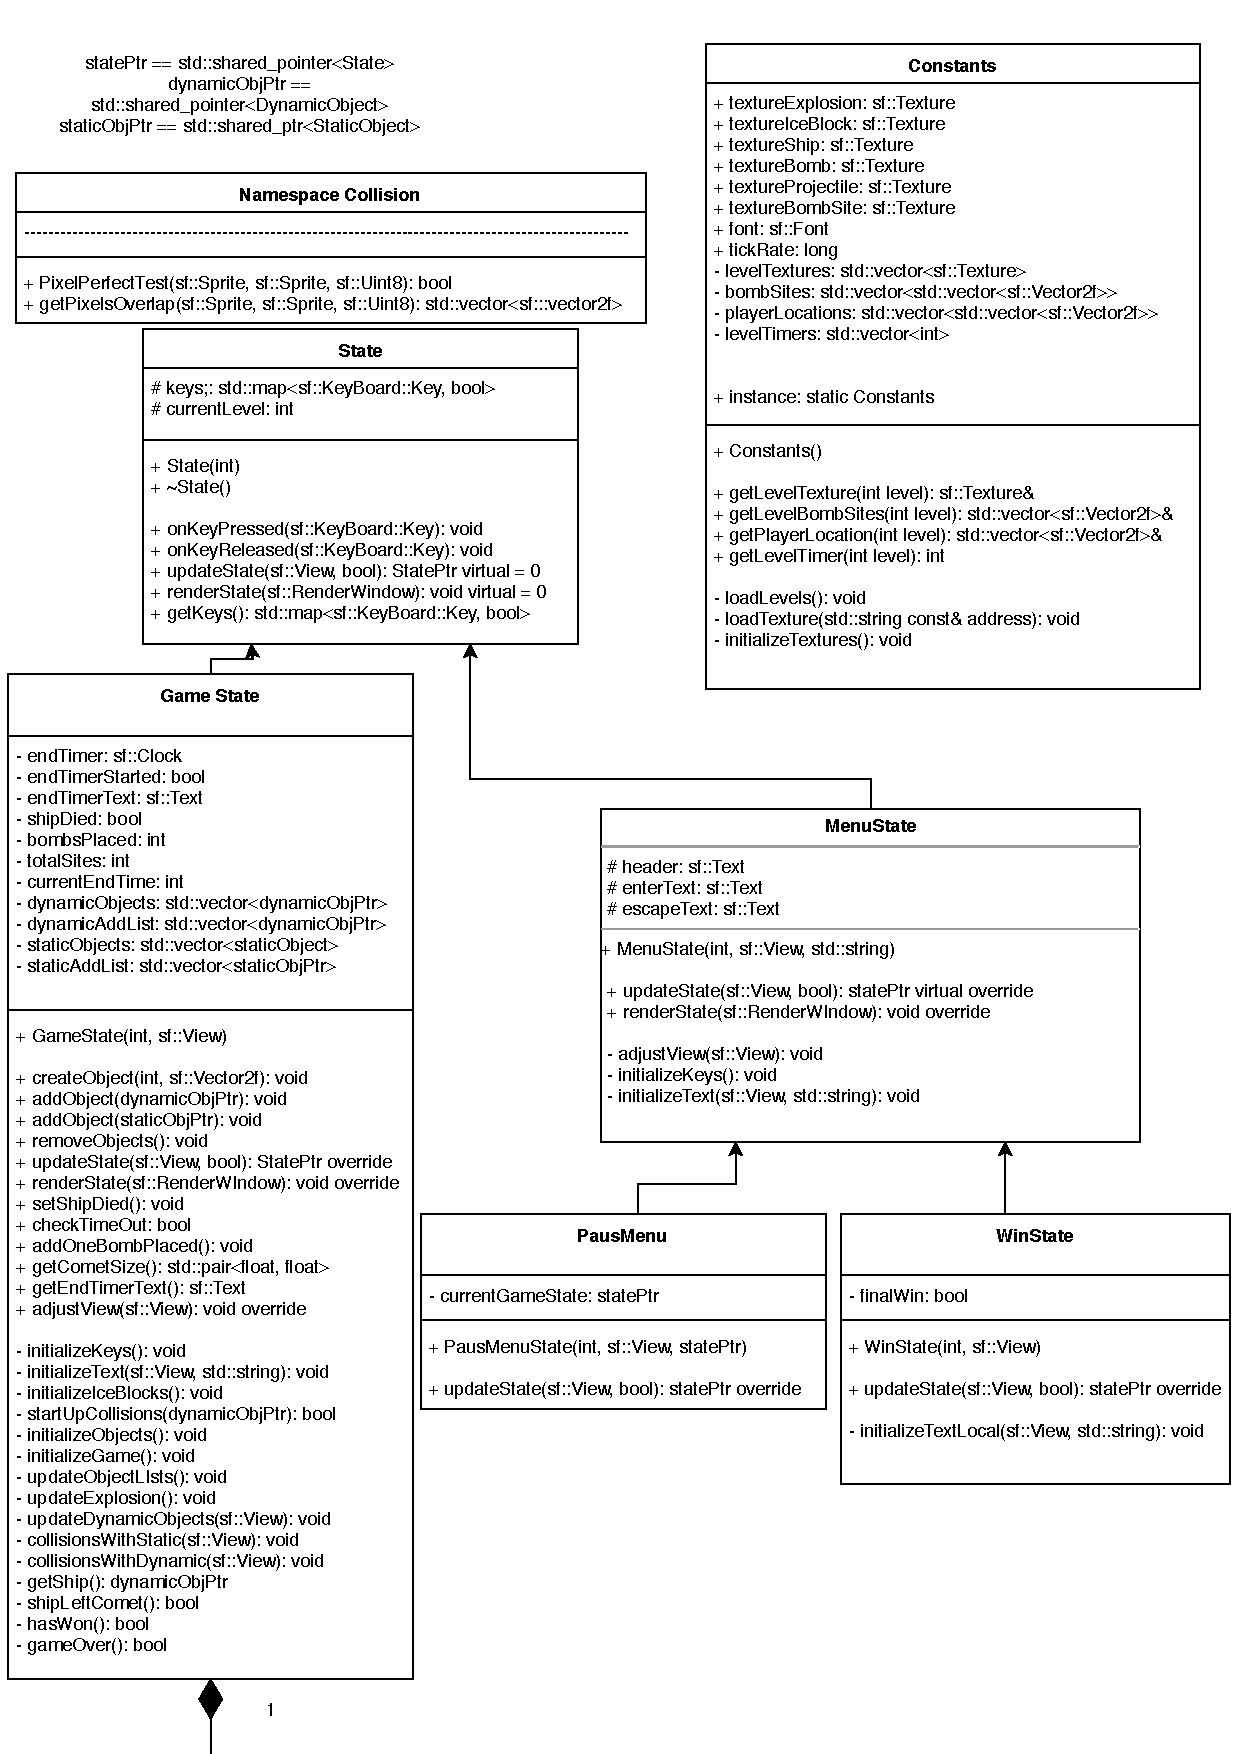
\includepdf[pages={1}, scale = 0.9]{tdp005-uml.pdf}
  \end{figure}
\pagebreak

\begin{figure}[h!]
  \includepdf[pages={2}, scale = 0.9]{tdp005-uml.pdf}
  \end{figure}
\pagebreak

\section{Detaljbeskrivning av klasser}
Nedan föjer detaljbeskrivningen av klasserna IceBlock och Ship. Dessa två valdes
då det är de två objekt som spelaren kommer komma i mest direkt kontakt med.
Ship i egenskap av det är farkosten som spelaren kontrollerar och IceBlock
eftersom det är spelarens huvudprövning.

Den fullständiga dokumentationen av spelets klasser finns generarat som html dokument via Doxygen
här. \url{html/index.html}

\subsection{Ship}
Ship är en inplementation av DynamicObject som i sin tur är en specialisering av
Object.

I Object klassen ingår medlemsvariablerna sprite som är en instans av SFML´s sf::Sprite
samt en bool variabel alive som anger om objektet är "vid liv" eller inte.
Vidare ingår medlemsfunktionerna:\\
isAlive()\\
Returnerar en bool om objectet är levande eller inte.\\
getSprite()\\
Returnerar objektets sprite.\\
draw()\\
Ritar ut objektets sprite på skärmen.\\
För detaljerad info om dessa medlemsfunktioner se
\url{html/classObject.html}

I DynamicObject ingår medlems variablerna mass: float, 
direction: sf::vector2f, speed(float), orientation: sf::Vector2f och 
radius: float.\\
DynamicObject ansvarar även för att hantera eventuella kollisioner avgöra om objektet är
levande eller inte samt updatera objektets position och orientation i banan.
För detaljerad information om DynamicObject klassen se klassdiagrammet oven eller den
detaljerade dokumentationen här \url{html/classDynamicObject.html}

Utöver ovannämnda variabler och funktioner i föräldraklasser har den faktiska 
Ship klassen variabler för att mäta liv (hp) och sköld hp (shieldHp) samt en variabel för hur
snabbt den kan accelerera och rotera. Vidare har Ship variabler för hur många bomber den har
kvar att spendera samt sf::Text variabler för att visa information om ovanstående variablers
status. 

skeppet har även egna updaterings funktioner för att uppdatera speed, direction, orientation,
updatera hp och shield hp, texter samt en funktion för att avfyra skeppets vapen.
\url{html/classShip.html}

\subsection{IceBlock}
IceBlock har samma föräldraklasser som Ship och ärver därmed samma variabler, 
för information om dessa se rubriken Ship.

Även IceBlock klassen har hp och när ett objekt av denna typ når noll hp så splittras det i två
eller tre mindre objekt beroende på dess massa ansvaret för att dela sig ligger i IceBlock
klassen. när två IceBlock objekt kolliderar så slås de samman genom en inelastisk kollision.
Ansvaret för denna operation ligger hos DynamicObject och en sådan kollision resulterar i att
deras massor slås samman och från massan kommer blockstorlek räknas ut.
\url{html/classIceBlock.html}

\pagebreak 
\section {Diskussion}
Nedan följer ett diskussionskapitel som innehåller designval samt vilka externa 
filformat som systemet ska använda sig av.

\subsection{Designval}
Genom att dela upp våra klasser som vi gjort har vi en relativt platt
struktur av beroenden med tydlig indelning i vad som är vad och hur det hänger
ihop. Vi har aktivt undvikit situationer där vi får dubbelt arv. Alla arv följer
linjärt på varandra. Nackdelen är att vi får långa if else if satser. Vi hade kunnat undvika
dessa genom att lägga mer funktionalitet längre ned i hierarkierna. Dock så hade vi istället
fått duplicering av funktionalitet. Eftersom spelet är relativt litet så togs beslutet att
eventuell belastning i runtime av spelet på grund av dessa if else if satser var liten i
förhållandet till tiden det skulle ta att skriva specialicerade lokala updatefunktioner i
varje klass.

Beslutet att göra en egen klass för att hålla alla konstanta variabler och alla texturer i spelet
togs då det löste problem vi fick med segmentation fault när objekt dog, samt det löste ett lagg
problem vi hade när explosionsanimationen lästes in från fil vid varje explosion.

\subsection{Externa filformat}
All grafik i spelet  består av Png filer som importeras till klassen Constants och laddas
därifrån till de sprites som ska he dem. Valet av Png är för att Png kan komprimeras
utan stora förluster av data dvs., oavsett hur många gånger vi komprimerar eller
läser våra filer kommer vi inte förlora information lagrade i dem.

En annan fördel är att formatet har en bred färgpalett som stödjer många format.
Detta innebär att vi fick väldigt fin grafik med lite tid och energi lagd på
design av bilder.

Sista relevanta fördelen med Png är att det formatet stödjer genomskinlighet
vilket underlättar när vi skapar bilderna och det bidrar till spelets
slutgiltiga "finish" grafiskt sätt.

Den stora nackdelen med Png dock är att filformatet kräver större lagringsutrymme.
vilket orsakade lagg när många explisioner lästes in samtidigt detta löstes med vår Constants
klass (se ovan).

Vi har även en txt fil där banspecifik information finns. Denna fil är strukturerad på så vis
att varje bana har en rad i dokumentet och all information läses in av en load funktion i
klassen Constants.\\

Exempel på hur filen LEVELS.txt ser ut:\\
// Adress***********time****player*******bombcoords ->\\
images/Bana1.png****120*****396*1446*****500*550*****1275*550*****2025*1075\\
ersätt * med blanksteg.\\

\end{document}
